\documentclass{article}
\usepackage{graphicx}
\usepackage{hyperref}
% \usepackage[UTF8]{ctex}


\begin{document}

    \title{Image Compression Using SVD Methods}
    \author{SX1916115 Jingtang Zhang}
    \date{2019-12-09}

    \maketitle

    \newpage

    \begin{abstract}
        SVD (Singular Value Decomposition)
        is one of the most important decomposition methods for matrix
        and is wildly used in signal processing and statistics.
        In this project, I’d like to analyze an application of
        SVD in image compression in computer science aspect.
        \par\textbf{Keywords: } Singular Value Decomposition; Image Compression
    \end{abstract}

    \section{Background}

        \subsection{Images Represented in Computers}
            \par
            Inside the computer, the images are represented by pixels.
            For a two-dimension image,
            the pixels are organized as an two-dimension array.
            For a basic greyscale image,
            each pixel’s value is an 8-bit integer ranging from 0-255,
            which describes how black the pixel is.
            \par
            For a colored image, each pixel needs more room to be represented.
            Generally, each pixel contains three color dimensions: 
            red (R), green (G) and blue (B),
            each dimension is represented in an 8-bit integer. 
            So, a colored pixel needs a storage of 24-bit.
            For an image with resolution of 1920 * 1080,
            it need a storage of 5.93MB.

        \subsection{Image Compression}
            \par
            Internet is becoming a necessary part of our daily life,
            within which multi-media traffic
            makes up the main part of the data traffic,
            through the sharing of photos and videos in social-network.
            Since the bandwidth of network is limited,
            users hope the transferring process to be faster,
            so that they will not be waiting for so long.
            However, the service provider cannot guarantee the stability
            of user’s network speed,
            a common way is to reduce the amount of data
            transferred through compressing the images.
            By compressing the image, sending it through the network,
            and decompressing the image at client side,
            the service providers can reduce the data transferred
            at the cost of a little bit more CPU computing resource,
            which is acceptable.
            \par
            In another case,
            for a photo which is taken by a professional photographer
            with his advanced camera,
            the resolution can be up to $3840\times2160$ pixels.
            However, for a mobile phone user with a 720p screen,
            say, with resolution of $1280\times720$ pixels,
            it is not necessary to display such a clear image.
            As a result, a compression is also needed.
            \par
            Generally, there are two categories of methods
            of image compression,
            based on whether there will be a loss of data after compression.
            But the goal of compression is the same:
            to represent an image with less data.
            SVD is one of the methods for compressing an image.

        \subsection{SVD}
            \par
            In linear algebra, the singular value decomposition (SVD)
            is a factorization of a real or complex matrix.
            It is the generalization of the eigen decomposition
            of a positive semidefinite normal matrix
            (for example, a symmetric matrix with non-negative eigenvalues)
            to any $m \times n$ matrix via an extension of
            the polar decomposition.
            It has many useful applications in signal processing and statistics.
            \par
            In detail, Suppose $M$ is an $m \times n$ matrix
            whose entries come from the field $K$,
            which is either the field of real numbers
            or the field of complex numbers.
            Then the singular value decomposition of M exists,
            and is a factorization of the form: $M = U \Sigma V^\mathrm{ H }$,
            where $U$ is an $m \times m$ unitary matrix over $k$.
            $\Sigma$ is a diagonal $m \times n$ matrix
            with non-negative real numbers on the diagonal,
            $V$ is an $n \times n$ unitary matrix over $K$,
            and $V^\mathrm{ H }$ is the conjugate transpose of $V$.
            \par
            Specifically, the column vectors of $U$ and $V$
            are two standard orthogonal basis, respectively.
            And each diagonal element $\sigma$ in $\Sigma$
            represents the stretch relationship.
            Bigger the diagonal element,
            more important the dimension is.


    \section{Motivation}
        \par
        Consider a real case:
        suppose we have an HD image with a resolution of $1920 \times 1080$ pixels.
        The image is represented in the memory in a two-dimension array (a matrix).
        If I want to transfer this image through network without compression,
        we need to send $1920 \times 1020 \times 8$ bytes of data,
        supposing the image is represented in the standard RGB-form.
        We decompose the matrix of the image $M$ of $1920 \times 1080$ with SVD method,
        where $U$ is a $1920 \times 1920$ matrix,
        $V^\mathrm{ H }$ is a $1080 \times 1080$ matrix,
        and $\Sigma$ is a $1920 \times 1080$ diagonal matrix.
        Specifically, most elements in $\Sigma$ are zero.
        \par
        Suppose the rank of $\Sigma$ is $k$.
        In order to recover $M$, only $k$ lines of $U$ and $V$ is needed,
        with $k$ elements of $\Sigma$.
        Thus, a total number of bytes to be
        transferred is: $$(1920 \times k + 1080 \times k + k) \times 8$$
        The ratio of compression is: $$\frac{1920 \times 1080}{(1920 + 1080 + 1) \times k} $$
        \par
        Moreover, since the value of some small non-zero diagonal elements are not so important
        compared with others, they can be ignored by regarding them as 0.
        Thus we get the most important $k'$ dimensions, which is smaller than k.
        As a result, we get a larger compression ratio,
        at the cost of losing $k - k'$ dimension of data while recovering.
        Smaller the k’, more dimension will be lost.
        However, in most cases, a loss of unimportant dimension is acceptable,
        considering the speed-up of transferring benefit from compression.
    

    \section{Implementation}
        \par
        I used OpenCV, an open source framework for image processing, to complete the experiment.
        Specifically, OpenCV provides out-of-the-box matrix implementation
        and SVD algorithm implementation. The source code is available at my GitHub:
            \url{https://github.com/mrdrivingduck/svd-image-compression}.
        \par
        I wrote a small program on an Surface book 2 laptop with an Intel i7-8650U CPU and 16GB RAM.
        The program read an image file into the memory as a matrix of $m \times n$,
        and used built-in SVD function to decompose the matrix into three matrix:
        \begin{itemize}
            \item $U$($m \times m$)
            \item $\Sigma$($m \times n$)
            \item $V$($n \times n$)
        \end{itemize}
        The matrix $\Sigma$ contains all singular values in descending order,
        while $U$ and $V$ contains orthogonal vectors corresponding to each singular value.
        \par
        Then, the program was given a compress ratio $r$,
        and it would only reserve the $r$\% most important singular value in $\Sigma$,
        and also, the corresponding vectors in $U$ and $V$ would be reserved.
        \par
        As for reconstructing the image,
        I copied the reserved singular values into the diagonal position of a zero-matrix $\Sigma'$.
        By multiplying $U$, $\Sigma'$ and $V$, we can get a compressed image.

    \section{Evaluation}
        \par
        I did an experiment using a real-world image.
        Specially, I showed the distribution of singular value after the compression,
        and evaluated the bandwidth saved by compression.
        Also, I used different values of $k'$ to see
        how the ignorance of dimensions affects on what an image looks like.

        \subsection{Distribution of Singular Value}
            \par
            I chose an image of $450 \times 800$,
            and used the aforementioned algorithm to get its singular value.
            \par
            I noticed that the singular values range in at most four magnitudes.
            The biggest singular value can be very big (50449.8),
            while the smallest can be under ten (7.94395).
            Intuitively, smaller singular values are not as important as bigger ones,
            thus would not play an important role while reconstructing the image.
            I simply ignored the smaller singular values according to the compress ratio $r$.

        \subsection{Bandwidth Saved by Compression}
            \par
            For an image of $m \times n$,
            the original pixels needed for transferring is: $$m \times n$$
            Here I suppose $m > n$.
            After compression, we have a diagonal matrix $\Sigma$ of $m \times n$,
            which can be reduced to $n \times 1$ because it is diagonal.
            Besides, we have two unitary matrices of $m \times m$ and $n \times n$, respectively,
            while $m \times m$ can be reduced to $m \times n$ because of zeros in $\Sigma$.
            Given the compress ratio $r$,
            the total cost is:
            $$(m \times n + n \times n \times n \times 1) \times r = n \times (m + n + 1) \times r$$
            \par
            When the $r$ is small enough, the bytes that should be sent can be saved greatly.
            The problem is, how small $r$ should be to effectively save the bandwidth,
            while maintaining what an image looks like originally by human eyes?

        \subsection{Effect of Different Compress Ratios}
            \par
            I used different compress ratios to see what the image looks like.
            A ratio of 0.3 means only 30\%
            the most important singular values (dimensions) are reserved.

            \begin{figure}[htbp]
                \centering
                \begin{minipage}[t]{0.45\linewidth}
                    \centering
                    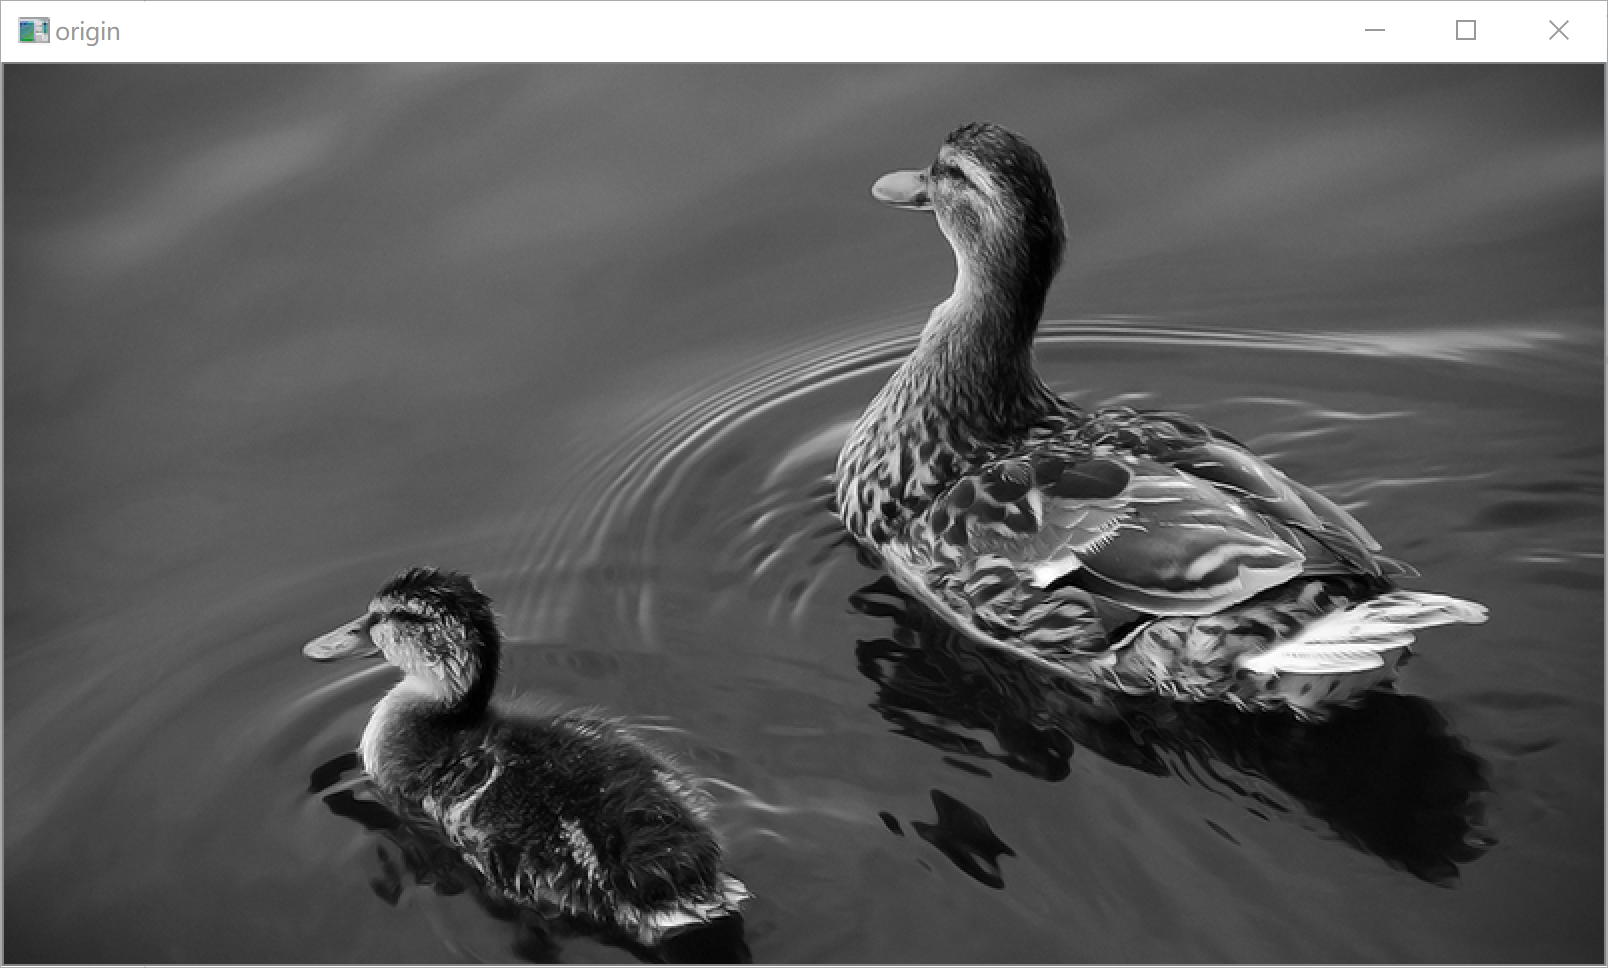
\includegraphics[height=2.8cm]{imgs/original.png}
                    \caption{Original Picture}
                \end{minipage}
                \hfill
                \begin{minipage}[t]{0.45\linewidth}
                    \centering
                    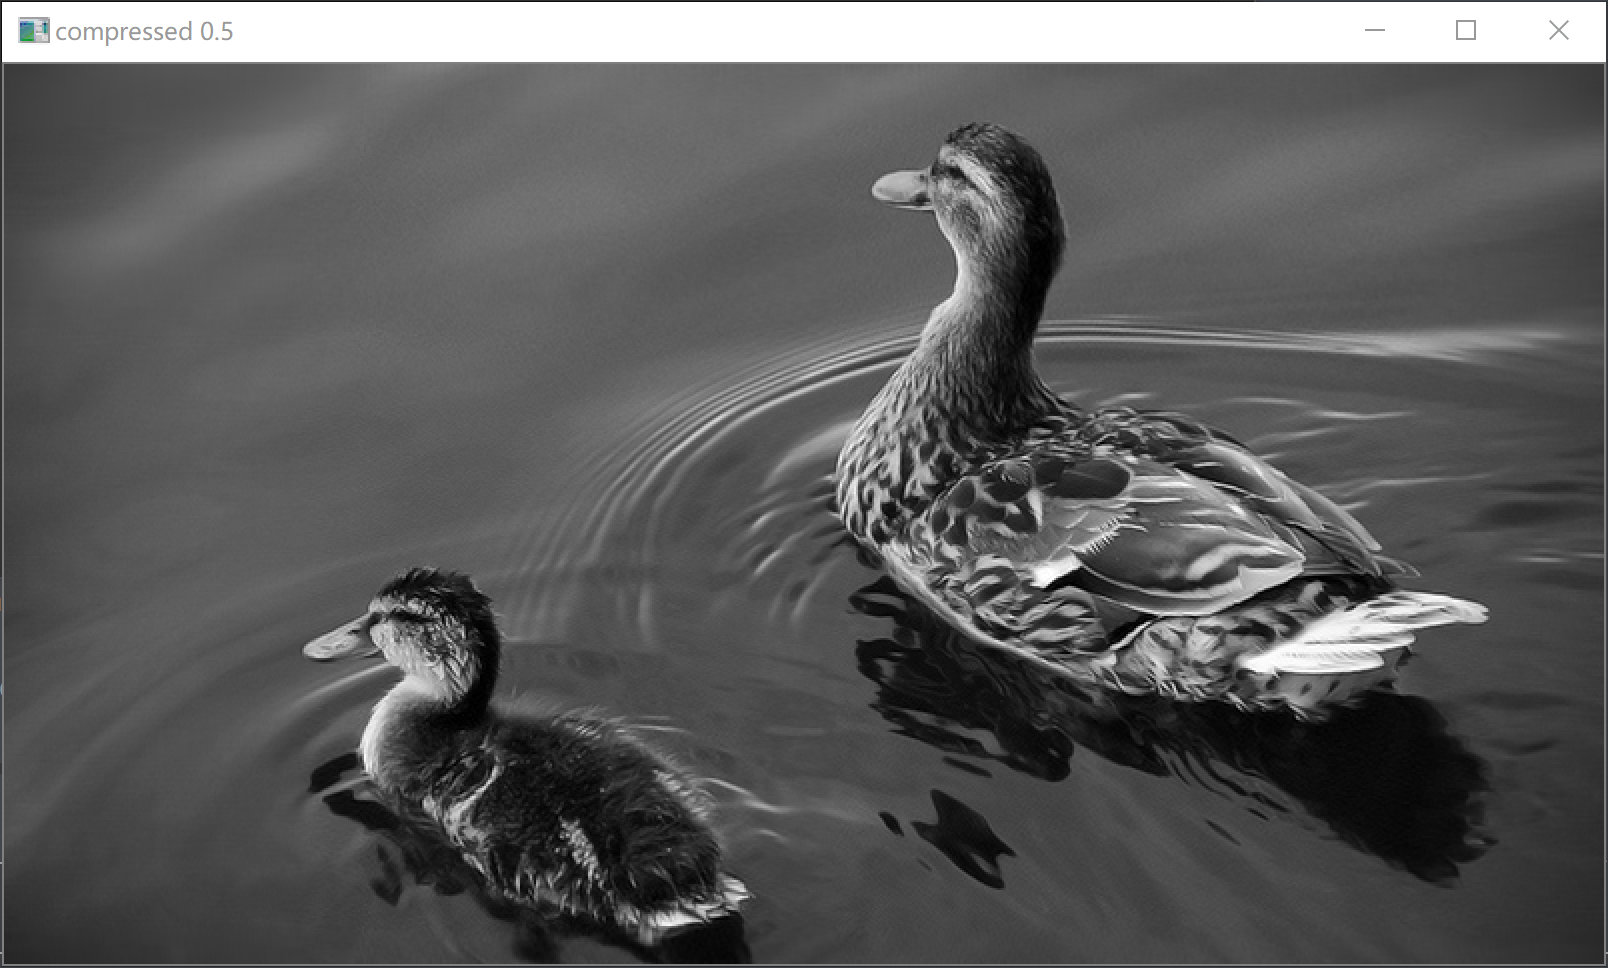
\includegraphics[height=2.8cm]{imgs/compressed-0.5.png}
                    \caption{50\% compress ratio}
                \end{minipage}
            \end{figure}
            \begin{figure}[htbp]
                \centering
                \begin{minipage}[t]{0.45\linewidth}
                    \centering
                    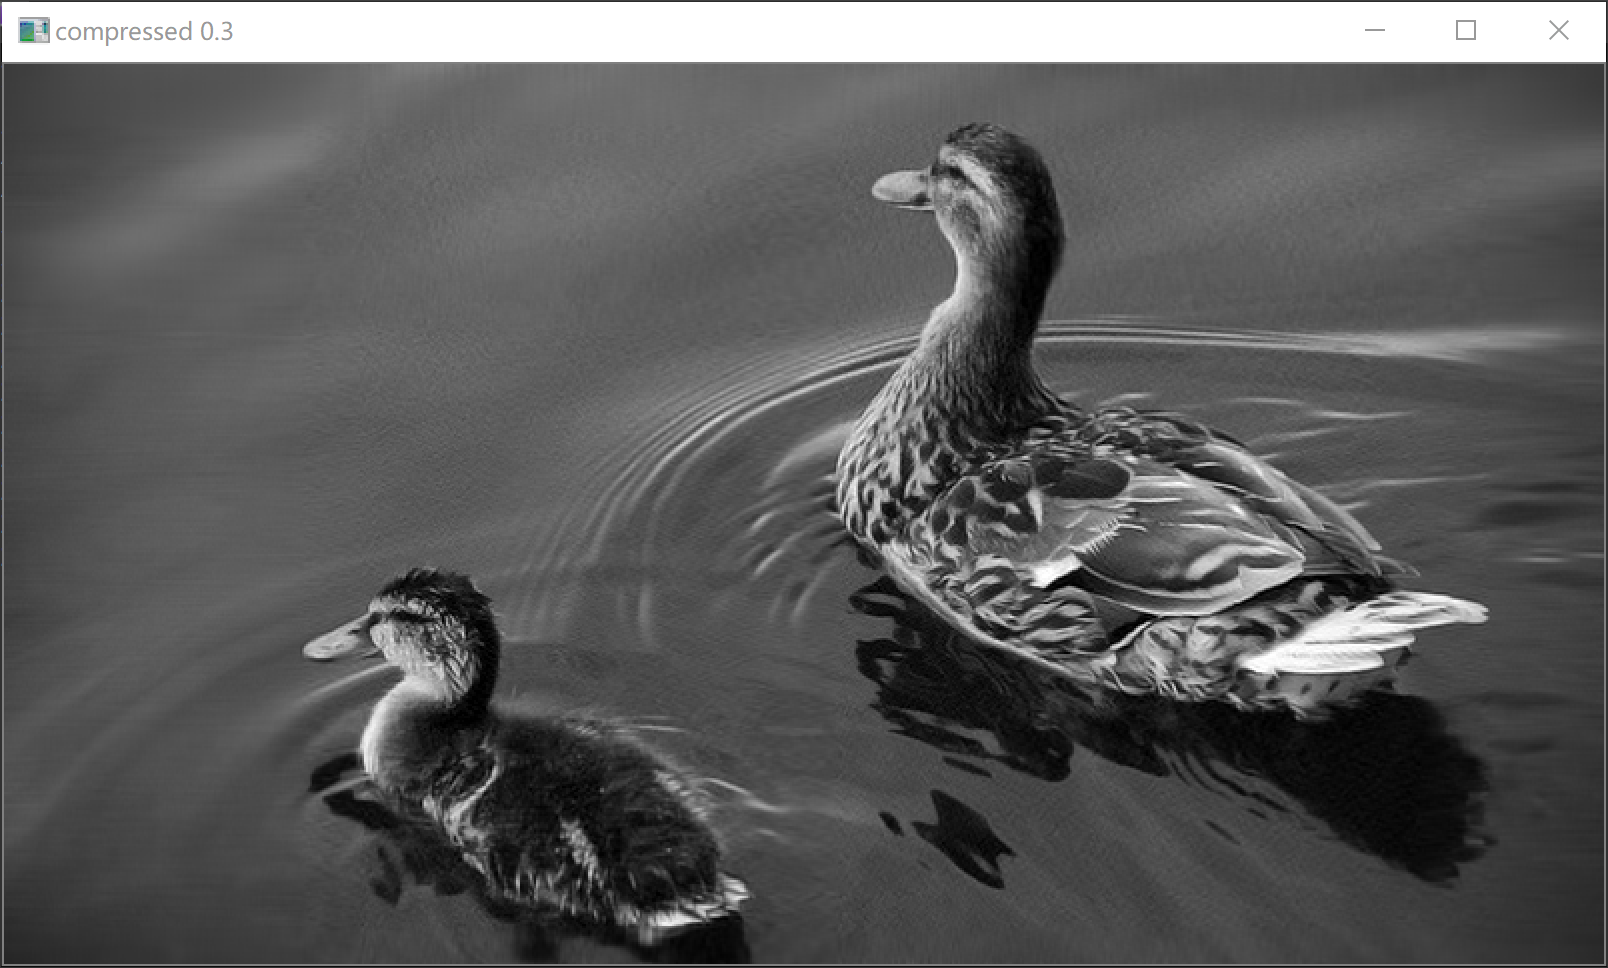
\includegraphics[height=2.8cm]{imgs/compressed-0.3.png}
                    \caption{30\% compress ratio}
                \end{minipage}
                \hfill
                \begin{minipage}[t]{0.45\linewidth}
                    \centering
                    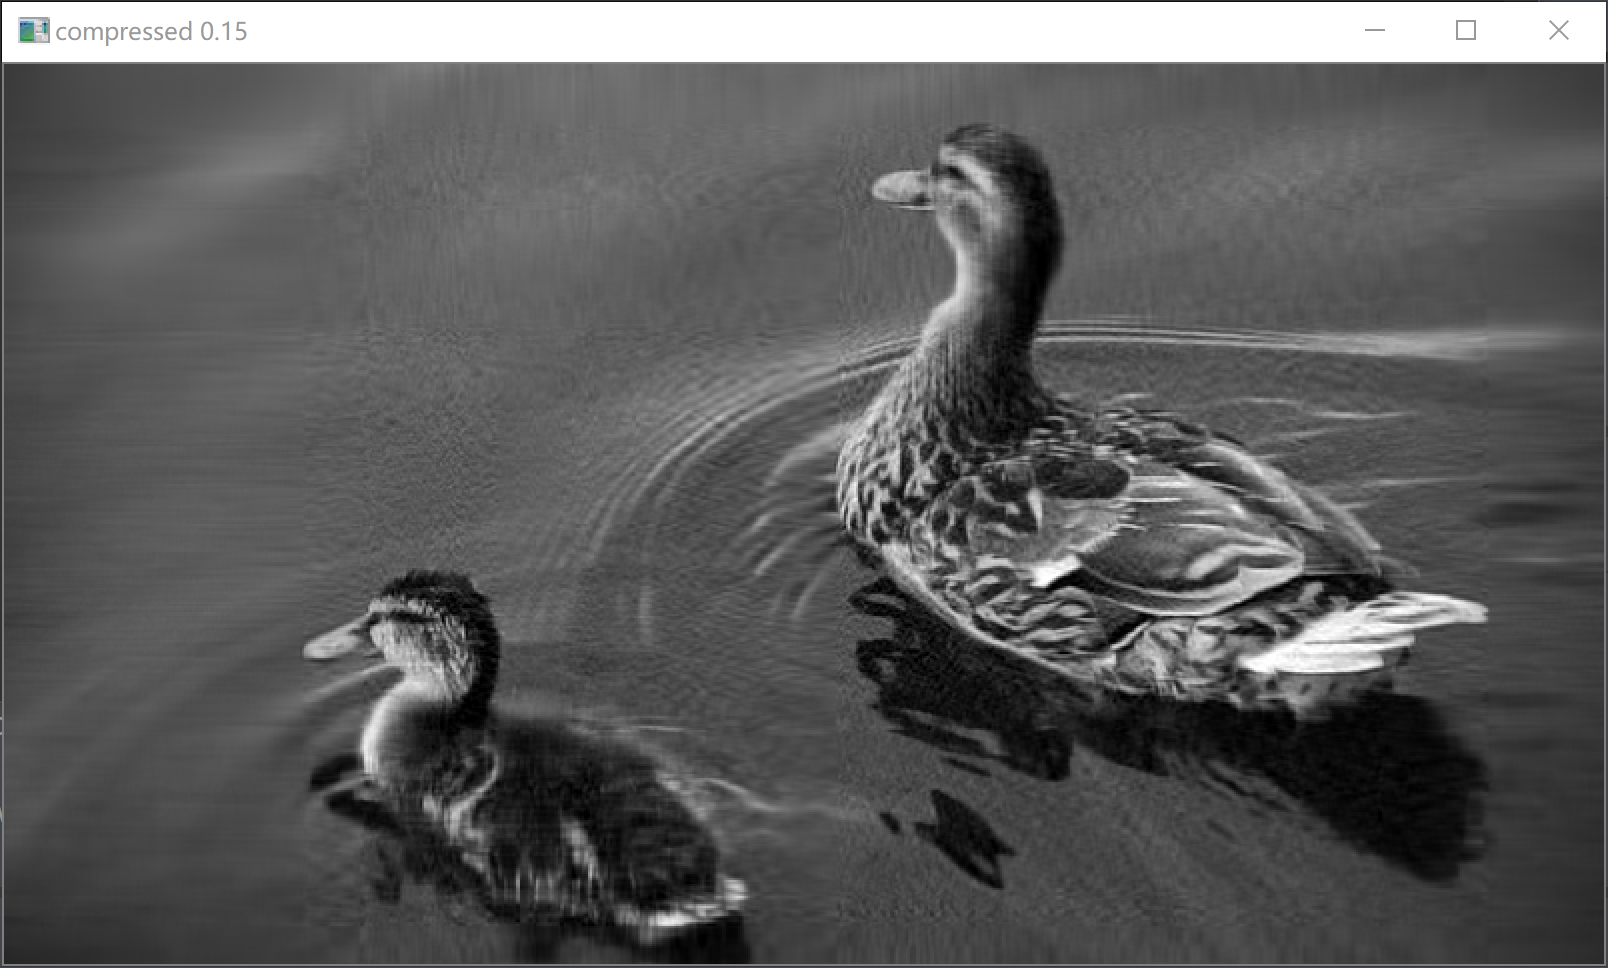
\includegraphics[height=2.8cm]{imgs/compressed-0.15.png}
                    \caption{15\% compress ratio}
                \end{minipage}
            \end{figure}
            \begin{figure}[htbp]
                \centering
                \begin{minipage}[t]{0.45\linewidth}
                    \centering
                    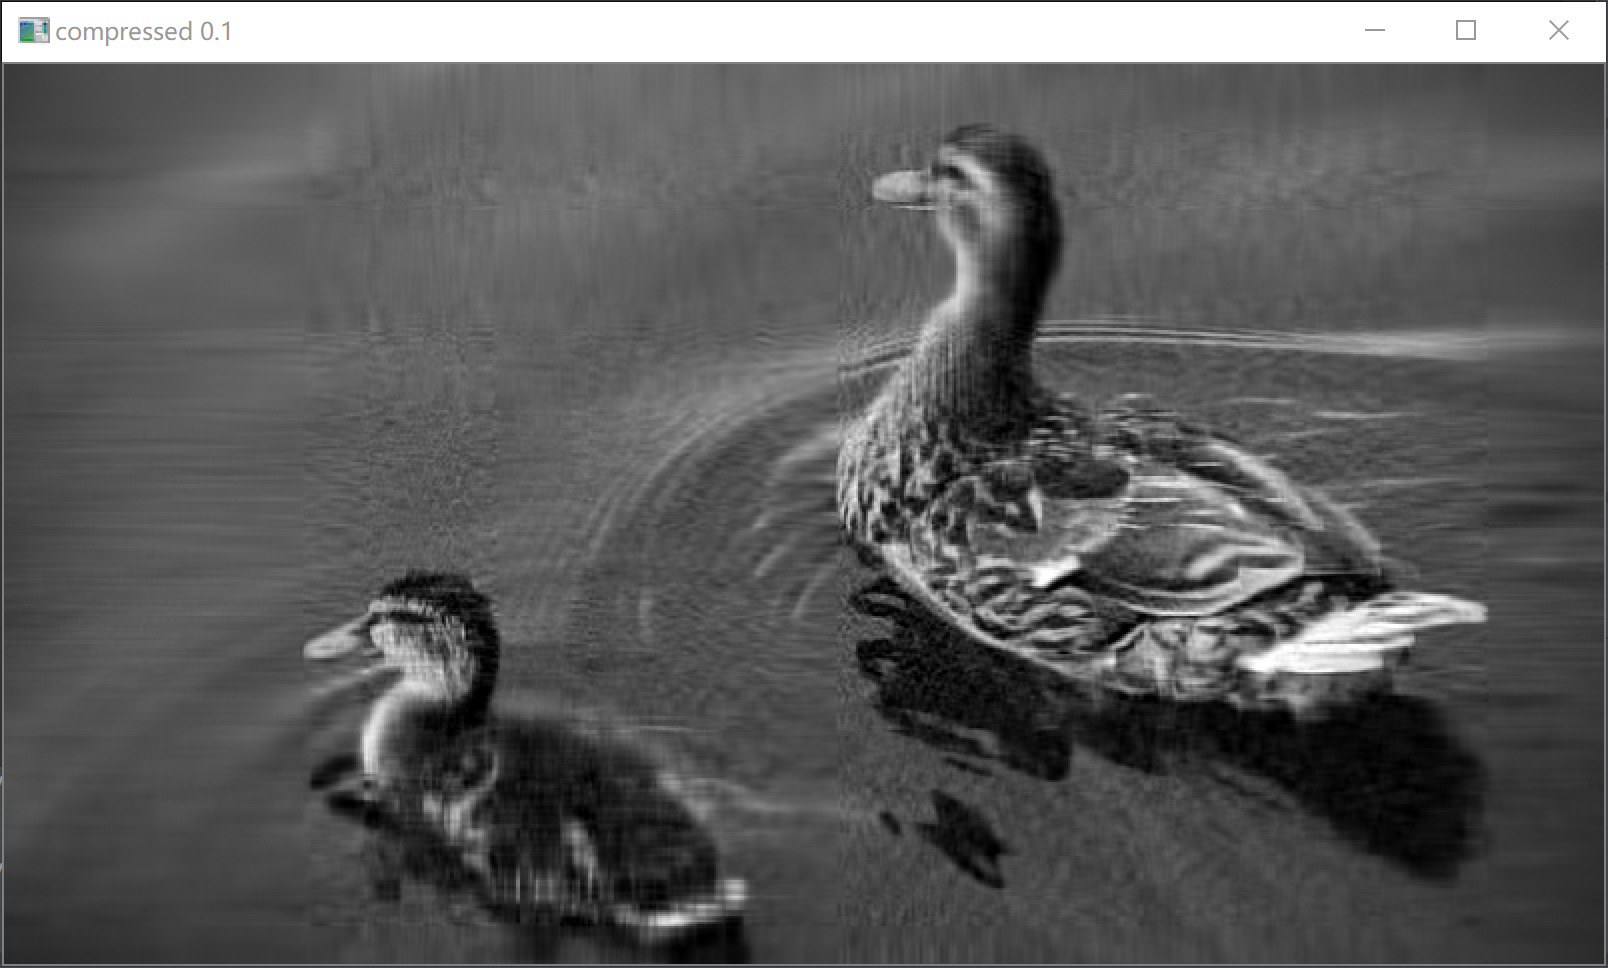
\includegraphics[height=2.8cm]{imgs/compressed-0.1.png}
                    \caption{10\% compress ratio}
                \end{minipage}
                \hfill
                \begin{minipage}[t]{0.45\linewidth}
                    \centering
                    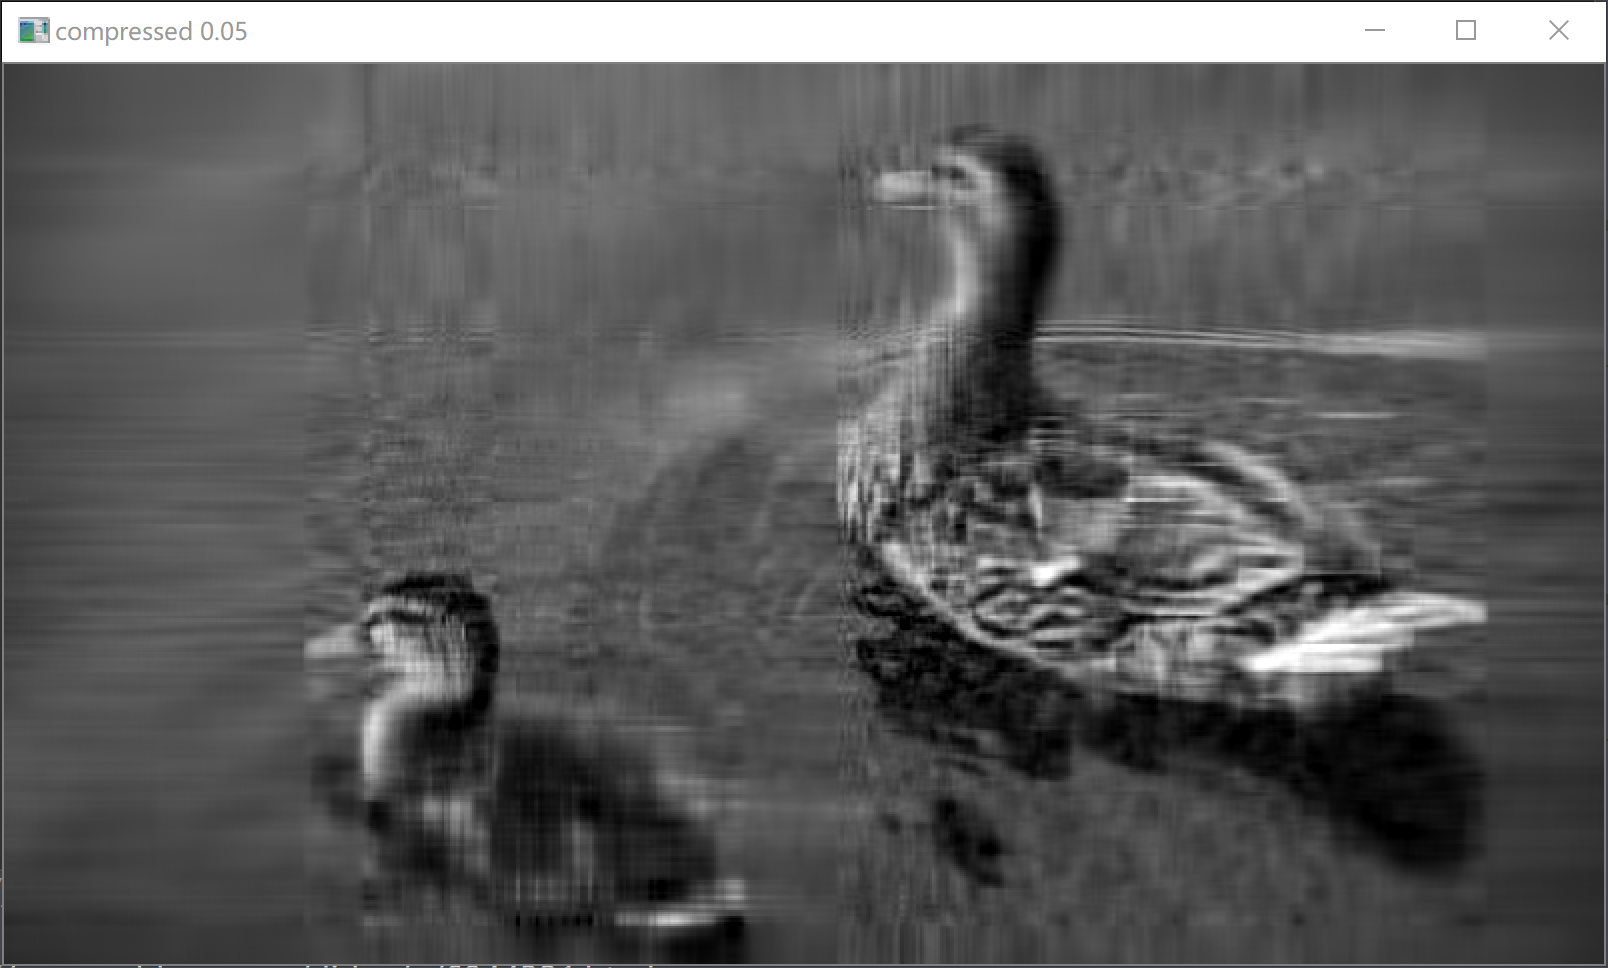
\includegraphics[height=2.8cm]{imgs/compressed-0.05.png}
                    \caption{5\% compress ratio}
                \end{minipage}
            \end{figure}

            \par
            It could be seen that: 30\% of the most important dimensions can reconstruct
            the image which is as clear as the original one for human eyes.


    \section{Conclusion}
        \par
        SVD is a useful method for image compression.
        It can save the bandwidth for the transfer of an image,
        while maintaining what the image looks like by human eyes.


\end{document}